%atmospheric O3 with budget, lifetime, stratospheric & tropospheric ozone
Ozone (\ce{O3}) is an atmospheric constituent gas found in the stratosphere and troposphere, however its atmospheric effects 
are very different in these distinct regions. About 90\% of the atmospheric ozone is present in the stratosphere, with a peak 
mixing ratio of about 12 ppm \citep{Seinfeld:2006}. Stratospheric ozone absorbs the sun's ultraviolet radiation in the 
wavelength region 280 - 315 nm, this is extremely important as excess UV radiation can cause skin cancer, cataracts and a 
suppressed immune system in humans and can also damage plant, single-cell organisms and aquatic ecosystems \citep{WMO:2010}. 

In contrast, tropospheric ozone that is found close to the surface is both a pollutant and a greenhouse gas. Increased levels 
of tropospheric ozone are harmful to humans, plants and other living systems, as high ozone exposure can lead to pulmonary 
problems in humans and can decrease both crop yields and forest growth \citep{WMO:2010}. The key component in Los Angeles 
photochemical smog was determined to be tropospheric ozone \citep{Haagen-Smit:1956}. 

Globally, tropospheric ozone is formed mainly via chemical production and downward transport from the stratosphere into the 
troposphere, called the Stratosphere-Troposphere Exchange (STE) may also play a role. The STE is driven by the Brewer-Dobson 
circulation \citep{Brewer:1949, Dobson:1956}.  This is a relatively slow circulation (over a timescale of weeks to months) and is
due to planetary wave disturbances in the troposphere \citep{Haynes:1991}. The circulation causes air to move downward from the 
stratosphere into the troposphere at the mid at high latitudes and is balanced by upward exchange at the tropics. The STE also 
has a seasonal variability where the maximum transport occurs during spring \citep{Appenzeller:1996}, due to the increase in 
altitude of the tropopause - the boundary level between the troposphere and the stratosphere - which moves stratospheric air 
into the troposphere. Hence, there is a maximum \ce{O3} transport into the troposphere during late winter and early spring.
The amount of tropospheric ozone accounted for by the STE is dependent on the  % continue from here
%only about 8\% of the total global budget \citep{Wang:1998}. Chemical loss 
%is the main sink of tropospheric ozone \citep{Wang:1998} whilst dry deposition accounts for 18\% of the global loss.  
%Tropospheric ozone has an average lifetime of about 22 days \citep{Wang:1998}, however this is dependent on latitude and time of
%year \citep{Stevenson:2006}.  

A spring-time peak in \ce{O3} concentration is common in many areas, especially in the midlatitude Northern Hemisphere, and it 
was originally thought that the STE was mainly responsible. However, it is only very rarely that \ce{O3} originating via STE 
can influence tropospheric \ce{O3} levels \citep{Lelieveld:2000}. It was later realised that this spring maximum is due to the
photochemical reactions occuring in the Northern Hemisphere spring after the buildup of reservoir species over winter 
\citep{Penkett:1986} that are then oxidised photochemically, the increase in these reactions is due to the increase in 
temperature, moisture and sunlight. Hence, photochemical reactions are the major source of surface tropospheric ozone 
\citep{Lelieveld:2000} and since \ce{O3} is produced in this way it is termed a secondary pollutant.

%meterology impacts 
Tropospheric \ce{O3} is not only impacted by emission levels, it is also affected by meteorological variables such as 
temperature, number of hours of sunshine and wind as these impact transport, wet deposition rates and also chemical reaction 
rates \citep{Hess:2009}. Meteorology influences both regional and global \ce{O3} \citep{Hess:2009}, climate patterns such as El 
Ni\~{n}o are also known to impact \ce{O3} levels in certain areas \citep{Sudo:2001}. El Ni\~{n}o can cause an increase in 
\ce{O3} in the 70$^{\circ}$E to 170$^{\circ}$E region is due to downward motion, suppressed convection and less water vapour, 
whereas the \ce{O3} decrease in the 170$^{\circ}$E to 70$^{\circ}$W region results from the opposite conditions.

The effect of meteorology is an aspect of atmospheric chemical transport modelling that needs to be taken into account. However
it is also frequently the major source of uncertainty for the calculated \ce{O3} concentrations. Wind speeds in particular may 
lead to under- or over-predicated values of \ce{O3} concentrations \citep{Sillman:1999}. 

Although the emphasis in this work is on photochemical model derived \ce{O3} prediction measures, there are ways of predicting 
\ce{O3} concentrations based on meteorological variables. There are statistical approaches to forecast the \ce{O3} 
concentration, the most common approach being multivariate linear regresson \citep{Comrie:1997}.  Neural networks can also be 
used to predict \ce{O3} concentrations, although as described in \citep{Comrie:1997} they give is no significant improvement 
from multivariate linear regression techniques.

In general, there is great effort to reduce anthropogenic emissions that impact air quality and human health. For example, the 
EPA in the US and European Union all have regulations related to air quality with a set exceedance limit for \ce{O3} 
concentrations. Many cities in the US, especially in the northeast and southern California, have reduced the emissions of 
\ce{O3} precursors - mainly volatile organic compounds (VOC) emissions - due to repeated exceedances \citep{Fiore:1998}. These 
VOC emission reductions have proven successful as the amount of \ce{O3} in these metropolitan areas has been decreased despite 
nitrogen oxide levels, which also impact \ce{O3} levels, being almost constant \citep{Fiore:1998, Lin:2001}.

Modelling of \ce{O3} has greatly influenced the understanding of complexity of atmospheric chemistry, for example the 
non-linear relationship of \ce{O3} production on the VOC and nitrogen oxides concentrations. This in turn has led to a better 
understanding on how to reduce the \ce{O3} levels for better air quality. The need for more realistic and effective air quality
standards in turn also drives the model development and deeper understanding of atmospheric chemistry. Providing detailed 
information of which VOCs can produce the most \ce{O3} is of greater benefit for regulation purposes rather than lumping all 
VOCs under one common regulation. Moreover, this can give indication on possibly replacement substances in order to improve air
quality.

An example is the modelling study in \citep{Capps:2010}, where an investigation into the effect of substituting less-reactive 
for more-reactive compounds. One consideration of the study was to establish whether there are also increased ozone 
concentrations due to atmospheric transport. It is shown that the more-reactive compounds do produce more ozone - in terms of 
mass - when compared to less-reactive compounds. Performing the same study using incremental reactivity scales (discussed in 
more detail in Section \ref{s:MIR&MOIR}) gives similar conclusions. Thus an investigation into the different ozone production 
pathways of VOCs can aid in substitution policies.

\section{Tropospheric Chemistry} \label{s:atmo_chem}

\subsection{Ozone Chemistry}
%O3 chemical sources & sinks, linking VOCs.
Troposperic ozone is principally formed by the photolysis of nitrogen dioxide (\ce{NO2}), which produces nitrogen oxide (NO) 
and a ground state oxygen atom (\ce{O(^3P)}), this then reacts with molecular oxygen (\ce{O2}) to form \ce{O3}. Ozone reacts 
rapidly with NO to return \ce{NO2} and \ce{O2}, this is represented by the following reaction cycle.
\begin{reactionlist}
    \reactionitem{\ce{NO2 + $h\upsilon$}}{NO + \ce{O(^3P)}}{new}{r:NO2photo}
    \reactionitem[M]{\ce{O(^3P) + O2}}{\ce{O3}}{new}{r:O3form}
    \reactionitem{\ce{NO + O3}}{\ce{NO2 + O2}}{new}{r:NO+O3}
\end{reactionlist}
These reactions do not produce net \ce{O3}, due to a photoequilibrium between NO, \ce{NO2} and \ce{O3} \citep{Atkinson:2000}. 
Adding VOCs of both biogenic and anthropogenic origin, such as methane (\ce{CH4}), and other gas-phase compounds, such as 
carbon monoxide (CO) - to the mix, results in net \ce{O3} production. The oxidation mechanism of CO, taking into account 
reactions that give maximum \ce{O3} yield, is
\begin{reactionlist}
    \reactionitem[\ce{O2}]{\ce{CO + OH}}{\ce{CO2 + HO2}}{new}{r:CO+OH}
    \reactionitem{\ce{HO2 + NO}}{\ce{NO2 + OH}}{new}{r:HO2+NO}
    \reactionitem{\ce{NO2 + $h\upsilon$}}{\ce{NO + O(^3P)}}{old}{r:NO2photo}
    \hline
    \reactionitem{Net: \ce{CO + 2O2 + $h\upsilon$}}{\ce{CO2 + O3}}{new}{r:netCO}
\end{reactionlist}
whilst the oxidation mechanism of \ce{CH4} with maximum \ce{O3} yield is
\begin{reactionlist}
    \reactionitem[\ce{O2}]{\ce{CH4 + OH}}{\ce{CH3O2 + H2O}}{new}{r:CH4+OH}
    \reactionitem[\ce{O2}]{\ce{CH3O2 + NO}}{\ce{HCHO + HO2 + NO2}}{new}{r:CH3O4+NO}
    \reactionitem[\ce{2O2}]{\ce{HCHO + $h\upsilon$}}{\ce{2HO2 + CO}}{new}{r:HCHOphotoa}
    \reactionitem{3(\ce{HO2 + NO}}{\ce{NO2 + OH})}{old}{r:HO2+NO}
    \reactionitem[\ce{O2}]{4(\ce{NO2 + $h\upsilon$}}{\ce{NO + O(^3P)})}{old}{r:NO2photo}
    \hline
    \reactionitem{Net: \ce{CH4 + 8 O2}}{\ce{CO + H2O + 2 OH + 4 O3}}{new}{r:netCH4+CO}
\end{reactionlist}
taking into account the net result for the CO oxidation mechanism \reactionref{r:netCO}, the net yield for \ce{CH4} is
\begin{reactionlist}
    \reactionitem{\ce{CH4 + 10 O2}}{\ce{CO2 + H2O + 2 OH + 5 O3}.}{new}{r:netCH4}
\end{reactionlist}
Both mechanisms are taken from \citep{Seinfeld:2006}.

To summarise, oxidation of VOCs results in the formation of peroxy radicals which then convert NO to \ce{NO2} and both 
\reactionref{r:NO2photo} and \reactionref{r:O3form} proceed. These oxidation mechanisms are linked in the sense that the 
\ce{CH4} mechanism gives a maximum \ce{O3} yield, once the mechanism of CO is also included. 

Since these mechanisms produce the maximum \ce{O3} yield, the reactions that cause \ce{O3} destruction or inhibit its 
production are not included. It should also be noted that some reactions can follow more than one pathway that is indicated 
above and that products from these pathways can be removed from the atmosphere via deposition processes. Thus, the maximum 
\ce{O3} yield outlined in reactions \reactionref{r:netCO} and \reactionref{r:netCH4} is not reached in the atmosphere.

Another aspect of \ce{O3} production is its dependence on the atmospheric concentrations of both VOCs and nitrogen oxides 
(\ce{NO_x = NO + NO2}) and this also influences the reaction pathways. Moreover, the precursors of ozone are linked to 
anthropogenic activity, hence a so-called weekend effect (i.e. there is a reduction on \ce{O3} concentration over the weekend) 
is also evident (see for example, \citep{Koo:2012}). Further discussion on the balance of VOC and \ce{NO_x} concentration to 
\ce{O3} production shall be given in Section \ref{s:VOC&NOx}.

\subsection{Chemical Families}

A concept that is extremely useful in atmospheric chemistry is that of a chemical family. This is used to describe two or more 
compounds that form a rapid cycle of production and destruction. An example is the cycling between NO and \ce{NO2} in 
\reactionref{r:NO2photo} and \reactionref{r:NO+O3}, hence NO and \ce{NO2} form the nitrogen oxides chemical family \ce{NO_x}.

A chemical family also has its own chemical lifetime, where the chemical lifetime is the average time that a chemical species 
takes to be removed - by reaction or deposition processes - from the atmosphere. An equilibrium is reached for the compounds of
the chemical family, called a pseudo-steady state, which is then re-balanced when a compound from the family reacts with a 
species not present in the chemical family.

Examples of important chemical families are given below in Table \ref{t:chemfam} and taken from \citep{Seinfeld:2006}.
\begin{table}
    \begin{center}
        \begin{tabular}{lll}
            \hline \hline
            \textbf{Symbol} & \textbf{Family Name} & \textbf{Components} \\
            \hline \hline
            \ce{NO_x} & Nitrogen oxides & NO + \ce{NO2} \\
            \ce{O_x} & Odd oxygen & \ce{O3 + O + O(^1D) + NO2 + NO3 + N2O5} \\
            \multirow{2}{*}{\ce{NO_y}} & \multirow{2}{*}{Oxidised nitrogen} & \ce{NO + NO2 + HNO3 + N2O5 + ClONO2} \\
            & & \hspace{0.5cm} \ce{ + NO3 + HOONO2 + BrONO2} \\
            \ce{HO_x} & Hydrogen radicals & \ce{OH + HO2} \\
            PAN & Peroxyacyl nitrates & Compounds of general formula \\ 
            & & \hspace{0.5cm} \ce{RC(O)OONO2} \\
            \hline \hline
        \end{tabular}
	\caption{Chemical Families commonly used in Tropospheric Chemistry \citep{Seinfeld:2006}}
	\label{t:chemfam}
    \end{center}
\end{table}

\subsection{Reservoir Molecules} \label{s:reservoir}

Compounds that react with radicals or \ce{NO_x} are called reservoir molecules. These will slow down \ce{O3} production and if 
they have a sufficiently long enough lifetime, can also transport and then release radicals or \ce{NO_x} to promote \ce{O3} 
formation in a separate location. For example, hydrogen peroxide (\ce{H2O2}) is a reservoir molecule for \ce{HO_x} as shown in 
the below sequence of reactions \citep{Seinfeld:2006}.
\begin{reactionlist}
    \reactionitem{\ce{HO2 + HO2}}{\ce{H2O2 + O2}}{new}{r:HO2+HO2}
    \reactionitem{\ce{H2O2 + $h\upsilon$}}{\ce{OH + OH}}{new}{r:H2O2photo}
    \reactionitem{\ce{H2O2 + OH}}{\ce{H2O + HO2}}{new}{r:H2O2+OH}
\end{reactionlist}

Nitrous acid (HONO) is a reservoir molecule for \ce{NO_x} and \ce{HO_x}, formed by a heterogeneous reaction of \ce{NO2} and 
\ce{H2O}. HONO can be formed during night-time and then photodissociates at sunrise to regenerate OH and NO 
\citep{Seinfeld:2006}.
\begin{reactionlist}
    \reactionitem{HONO + $h\upsilon$}{OH + NO}{new}{r;HONOphoto}
\end{reactionlist}

An important class of reservoir molecules are ther peroxyacyl nitrates (PANs) of general formula \ce{RC(O)OONO2}. The first 
compound in this class, \ce{CH3C(O)OONO2}, is also called PAN and can be formed by reactions of peroxyacetyl radicals with 
\ce{NO2}, PAN then thermally dissociates to return the reactants \citep{Kleinman:2005}.
\begin{reactionlist}
    \reactionitemrev{\ce{CH3C(O)O2 + NO2 + M}}{\ce{CH3C(O)OONO2 + M}}{new}{r:PANform}
\end{reactionlist}
PAN's lifetime is dependent on meteorology due to a strong temperature dependence \citep{Moxim:1996}. This can lead to 
situations where \ce{NO_x} is transported to different regions and then released by dissociation. PAN is thought to have a 
regional rather than a global influence on the \ce{NO_x} budget \citep{Moxim:1996}.

\subsection{Volatile Organic Compounds}
%VOCs to be considered
Table \ref{t:VOClist} lists Non-Methane Volatile Organic Compounds (NMVOCs) that are emitted from US cities \citep{Baker:2008}. 
The mean is calculated from \citep{Baker:2008} using the total of 31 data points from 28 cities in the United States. Of these 
NMVOCs there is only one which has a primarily biogenic source and this is isoprene (2-methyl 1,3-butadiene). Although not 
evident from Table \ref{t:VOClist}, biogenic VOCs are globally the most abundant VOCs \citep{Goldstein:2007}. Since the data in 
Table \ref{t:VOClist} are mainly taken from urban cities, the impact of anthropogenic emissions outweigh those of the biogenic 
sources \citep{Baker:2008} - although isoprene has some anthropogenic sources (see \citep{Borbon:2003}). 
\begin{table}
    \begin{center}
        \begin{tabular}{ll}
            \hline \hline
            \multirow{2}{*}{\textbf{Compound}} & \textbf{Mean Mixing} \\ & \textbf{Ratio (pptv)} \\
            \hline \hline \multicolumn{2}{c}{\textbf{Alkanes}}  \\ \hline
            Ethane & 2498 \\
            Propane  & 1449 \\
            Butane (n-butane) & 623 \\
            2-methyl propane (i-butane) & 386 \\
			Pentane (n-pentane) & 349 \\
            2-methyl butane (i-pentane) &771 \\
		    Hexane (n-hexane) & 137 \\
            Heptane (n-heptane) & 81 \\
            Octane (n-octane) & 41 \\ \hline \multicolumn{2}{c}{\textbf{Alkenes and Alkyne}} \\ \hline
            Ethene &789 \\
			Propene & 205 \\
            1-butene & 64 \\
            2-methyl propene (i-butene) & 200 \\
            2-methyl 1,3-butadiene (isoprene) & 760 \\
            Ethyne & 730 \\ \hline \multicolumn{2}{c}{\textbf{Aromatics}} \\ \hline 
			Benzene & 175 \\
            Methyl benzene (Toluene) & 572 \\
            1,3-dimethyl benzene (m-xylene) & 115 \\
            1,4-dimethyl benzene (p-xylene) & 61 \\
            1,2-dimethyl benzene (o-xylene) & 105 \\
			Ethyl benzene & 91 \\ \hline \hline
        \end{tabular}
    \end{center}
    \caption{NMVOCs emitted from US cities \citep{Baker:2008}} 
    \label{t:VOClist}
\end{table}

The sources of the alkanes listed below are natural gases, liquified petroleum gas (LPG), combustion and industry, for the case
of octane, vehicle exhaust is also a source. Alkene sources are mainly due to industrial activities and vehicular emissions. 
Aromatic compounds are mainly due to vehicle emissions, while benzene and toluene are also emitted due to industrial activity 
and combustion is also a further source for benzene \citep{Arsene:2009}.

%reactivity of species - Atkinson
Alkanes are saturated hydrocarbons, meaning that all bonds between carbon and hydrogen atoms are single bonds, resulting in 
slow reacting species. The dominant tropospheric process for alkanes is reaction with the hydroxyl (OH) radical, but they also 
react with the nitrate (\ce{NO3}) radical and chlorine atoms. The presence of a double bond in alkenes and a triple bond in 
alkynes leads to increased reactivity. In the troposphere both alkenes and alkynes react with the OH radical, the \ce{NO3} 
radical and also with \ce{O3}. Aromatic compounds react with the OH and \ce{NO3} radicals. Hence it can be noted that the key 
reactive species in the troposphere is the OH radical as it reacts with practically all organic compounds, the exceptions being
chlorofluorocarbons (CFCs) and halons without hydrogen atoms. 

Reaction with the OH radical is predominant during the day, since it is formed mainly by photolysis, during the night there is 
an increase in the \ce{NO3} radical concentration and so reaction rates with this radical are increased. The reason for this 
increased night-time concentration of the \ce{NO3} radical is that during the day the reaction that forms \ce{NO3} 
\begin{reactionlist}
    \reactionitem{\ce{NO2 + O3}}{\ce{NO3 + O2}}{new}{r:NO2+O3}
\end{reactionlist}
is balanced by the quick photolysis of \ce{NO3}
\begin{reactionlist}
    \reactionitem{\ce{NO3} + $h\upsilon$}{\ce{NO + O2}}{new}{r:NO3photoa}
    \reactionitem{\ce{NO3} + $h\upsilon$}{\ce{NO2 + O(^3P)}.}{new}{r:NO3photob}
\end{reactionlist}
The main photolysis pathway is via reaction \reactionref{r:NO3photob} which occurs about 90\% of the time. However, during 
night-time photolysis does not occur and hence there is a buildup of \ce{NO3} radicals \citep{Atkinson:1990, Atkinson:2000}.

\subsection{VOC Chemistry}
%atmospheric chemistry of NMVOCs 
Figure \ref{f:VOC_reaction} represents a general and simplified reaction scheme for VOCs in the troposphere. Although there are
many different VOC classes involved in tropospheric chemistry, there are many similarities between their reaction schemes. This
shall be summarised below however for more a more detailed description of tropospheric chemistry, \citep{Atkinson:2000} should 
be consulted. 
\begin{figure}
    \begin{center}
        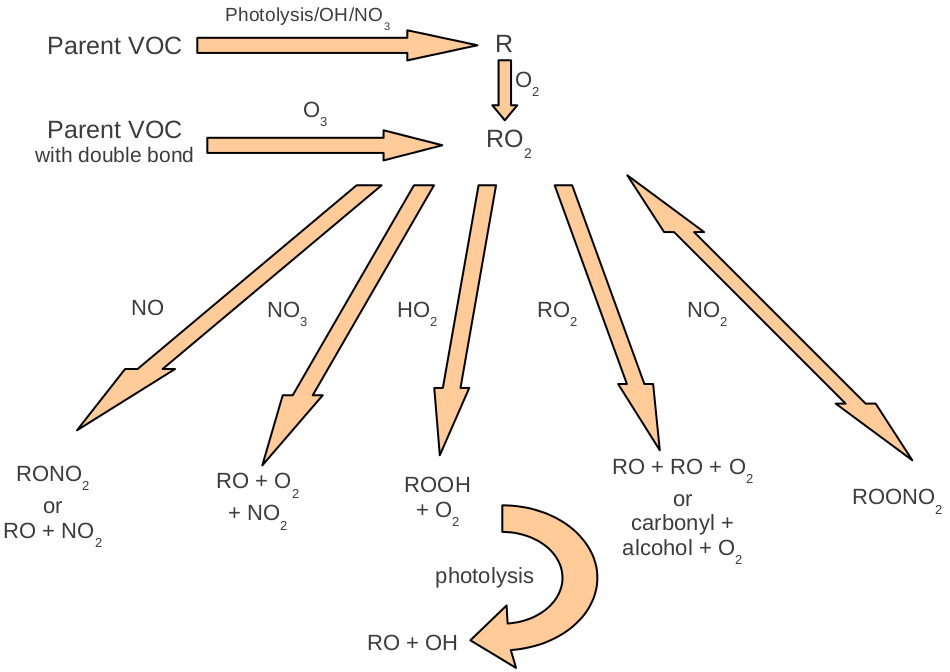
\includegraphics[height=100mm, width=120mm]{VOC_reaction_updated}
        \caption[what is this]{VOC reaction pathway}
        \label{f:VOC_reaction}
    \end{center}
\end{figure}

As noted earlier, the most common initiation reaction of a VOC is with the OH radical, and this forms an alkyl or substituted 
alkyl radical (R) depending on the parent VOC. The addition reaction with \ce{O2} then leads to the formation of alkyl peroxy 
radicals (\ce{RO2}). During the night-time, reaction with the \ce{NO3} radical is of importance and for VOCs containing a 
double bond, reaction with \ce{O3} also occurs. Photolysis is an important degradation initiator for carbonyl species, this is 
particularly important throughout the whole degradation mechanism of the VOC as carbonyl species, such as formaldehyde, are 
common reaction products. These initial reaction pathways all lead to the formation of \ce{RO2} radicals, as shown below.
\begin{reactionlist}
    \reactionitem{VOC + OH/\ce{NO3 / O3}/$h\upsilon$}{R}{new}{r:VOCinit}
    \reactionitem{R + \ce{O2}}{\ce{RO2}}{new}{r:R+O2}
\end{reactionlist} 
\ce{RO2} radicals can subsequently react with NO, \ce{NO2}, hydroperoxy (\ce{HO2}) radicals, \ce{NO3} radicals - mainly during 
night-time - and also with other alkyl peroxy radicals. The competition between these reactions determines the amount of net 
ozone production or loss from the parent VOC. 
\begin{reactionlist}
    \reactionitem{\ce{RO2 + NO + M}}{\ce{RONO2 + M}}{new}{r:RO2+NOa}
    \reactionitem{\ce{RO2 + NO}}{RO + \ce{NO2}}{new}{r:RO2+NOb}
    \reactionitemrev{\ce{RO2 + NO2 + M}}{\ce{ROONO2 + M}}{new}{r:RO2+NO2}
    \reactionitem{\ce{RO2 + HO2}}{ROOH + \ce{O2}}{new}{r:RO2+HO2}
    \reactionitem{\ce{RO2 + NO3}}{\ce{RO + NO2 + O2}}{new}{r:RO2+NO3}
    \reactionitem{\ce{RCH(OO)R$'$ + RCH(OO)R$'$}}{\ce{RCH(O)R$'$ + RCH(O)R$'$ + O2}}{new}{r:RCHOOR+RCHOORa} 
    \reactionitem{\ce{RCH(OO)R$'$ + RCH(OO)R$'$}}{\ce{RCH(OH)R$'$ + RC(O)R$'$ + O2}}{new}{r:RCHOOR+RCHOORb}
\end{reactionlist}
All pathways in Figure \ref{f:VOC_reaction} that lead to \ce{NO2} formation can result in \ce{O3} formation due to 
\reactionref{r:NO2photo} and \reactionref{r:O3form}. Reaction with the \ce{HO2} radical results in the formation of 
hydroperoxides (ROOH), which then photolyse to an alkoxy (RO) radical and the OH radical, this OH radical is then available to 
react with other VOCs. The carbonyl and alcohol products resulting from reaction with other \ce{RO2} radicals will follow a 
similar sequence of reactions and hence can also produce further \ce{O3}. Reaction with \ce{NO2} leads to the formation of 
alkyl peroxynitrates (\ce{ROONO2}), however this reaction product can be thermally unstable and may decompose quickly to the 
reactants, as mentioned in Section \ref{s:reservoir}.

The RO radical that results from many of the \ce{RO2} pathways undergoes further reactions, either by decomposition, 
isomerisation or reaction with \ce{O2}. The products that result from the reaction pathways depend on the parent VOC and this 
also determines the number of NO-to-\ce{NO2} conversions, eventually leading to \ce{O3} formation.

All VOCs and their degradation products will ultimately result in carbon dioxide (\ce{CO2}) and water vapour. The path that 
each VOC takes to reach its final products is dependent on the type of VOC, the radical concentration, the \ce{NO_x} 
concentration and other factors such as time of day and year. The detailed atmospheric chemistry of some simple VOCs is 
well-understood (for example, methane) however for more complex molecules, especially aromatic VOCs, there are a great number 
of uncertainties. These uncertainties can be related to kinetic data, photolysis rates, reaction branching ratios and in most 
cases the reaction products. Any uncertainties in reaction pathways and products of VOCs also leads to uncertainties in the 
ozone forming potential of the respective VOC \citep{Atkinson:2000}.

\subsection{\texorpdfstring{VOC and \ce{NO_x} Chemistry}{VOC and NOx Chemistry}} \label{s:VOC&NOx}
%balance of NOx & NMVOC for O3 production
As mentioned above, \ce{O3} chemistry is influenced by both VOC and \ce{NO_x} concentrations. Figure \ref{f:O3_isopleth} 
depicts the non-linear relationship between \ce{O3} concentration when considered as a function of VOC concentration (in ppmC, 
i.e. parts per million mass of a carbon unit of the VOC, \ce{CH_{2.5}}) and \ce{NO_x} concentration (in ppm, i.e. parts per 
million mass). 
\begin{figure}
	\begin{center}
		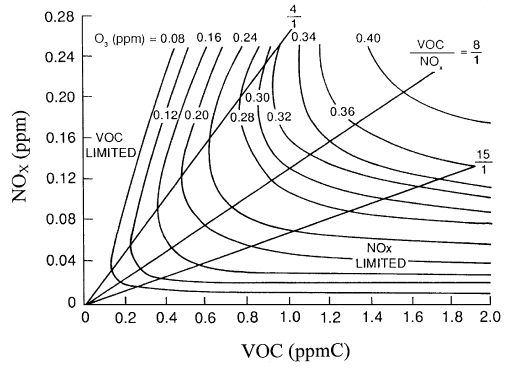
\includegraphics[height=90mm, width=85mm]{O3_isopleth_1.png}
		\caption{Ozone isopleth plots for various initial concentrations of \ce{NO_x} and a specified VOC mixture. Taken from \citep{Jenkin:2000}.}
		\label{f:O3_isopleth}
	\end{center}
\end{figure}

This relationship can be divided into distinct regimes: \textbf{\ce{NO_x}-sensitive}, \textbf{VOC-sensitive} and 
\textbf{VOC-and-\ce{NO_x}-sensitive}. The \ce{NO_x}-sensitive regime is the right-most part, the VOC-and-\ce{NO_x}-senstive 
regime is the middle section and the VOC-sensitive regime is the left-most part of Figure \ref{f:O3_isopleth} and these 
correspond to high, middle and low VOC:\ce{NO_x} ratios, respectively.  These different regimes arise from how the atmosphere 
removes \ce{NO_x} and radicals resulting from VOCs. 

In the \ce{NO_x}-sensitive regime, the concentration of \ce{NO_x} is low compared to that of radicals. Hence, peroxy radicals 
are removed by reaction with the OH radical such as 
\begin{reactionlist}
    \reactionitem{\ce{HO2 + OH}}{\ce{H2O + O2}}{new}{r:HO2+OH}
\end{reactionlist}
or by peroxy radical addition reactions.
\begin{reactionlist}
    \reactionitem{\ce{HO2 + HO2}}{\ce{H2O2}}{old}{r:HO2+HO2}
    \reactionitem{\ce{RO2 + HO2}}{\ce{ROOH + O2}}{old}{r:RO2+HO2}
\end{reactionlist}
This results in the NO concentration controlling the number of NO-to-\ce{NO2} conversions, rather than the concentration of 
peroxy radicals produced during VOC oxidation. An increase in NO conversion would thus promote \ce{O3} production due to an 
increase in \reactionref{r:NO2photo} and \reactionref{r:O3form} reactions. Increasing VOC concentrations would not increase 
\ce{O3} production as this only speeds up the formation of peroxy radicals and has no direct effect on the \ce{NO_x} 
concentration.

The VOC-sensitive regime corresponds to high \ce{NO_x} concentrations, hence radicals will tend to react with either NO or 
\ce{NO2}. Increasing \ce{NO_x} concentrations will not increase not increase \ce{O3} production as the \ce{NO_x} will react 
with the peroxy radicals resulting from VOC degradation. However, this increase in \ce{NO_x} increases the formation of nitric 
acid (\ce{HNO3}) by reaction with the OH radical \citep{Kleinman:1991, Kleinman:1994, Kirchner:2001}.
\begin{reactionlist}
    \reactionitem{\ce{OH + NO2}}{\ce{HNO3}}{new}{r:OH+NO2}
\end{reactionlist}
The competition of VOCs and \ce{NO_x} for reaction with the OH radical is at the heart of \ce{O3} production or destruction in 
the VOC-sensitive regime. Reaction of VOCs with the OH radical will produce more peroxy radicals, increasing \ce{O3} production
whilst reaction of \ce{NO_x} increases \ce{HNO3} by \reactionref{r:OH+NO2} which reduces \ce{O3} production 
\citep{Kleinman:1991, Kleinman:1994, Kirchner:2001}.

The VOC-and-\ce{NO_x}-sensitive regime is characterised by \ce{O3} production being sensitive to both VOC and \ce{NO_x} 
concentrations. The turning point from a VOC-sensitive to a VOC-and-\ce{NO_x}-sensitive regime is when the maximum \ce{O3} 
production for a particular VOC concentration has been reached. The shift into a \ce{NO_x}-sensitive occurs when increases in 
VOC concentrations result in very little \ce{O3} production \citep{Kirchner:2001}. The non-linear relationship can be thought of
as a titration process between the amount of radicals and the \ce{NO_x} present in the atmosphere.

This non-linear nature of the atmosphere must be taken into account when policymakers consider control strategies for \ce{O3} 
concentrations. The difficulty is exacerbated by the fact that regions can alternate between these regimes depending on the 
season, time of day etc. 

Moreover, an air parcel emitted in an urban area may also evolve as outlined in Figure \ref{f:air_parcel}, as it moves 
downwind. 
\begin{figure}
	\begin{center}
		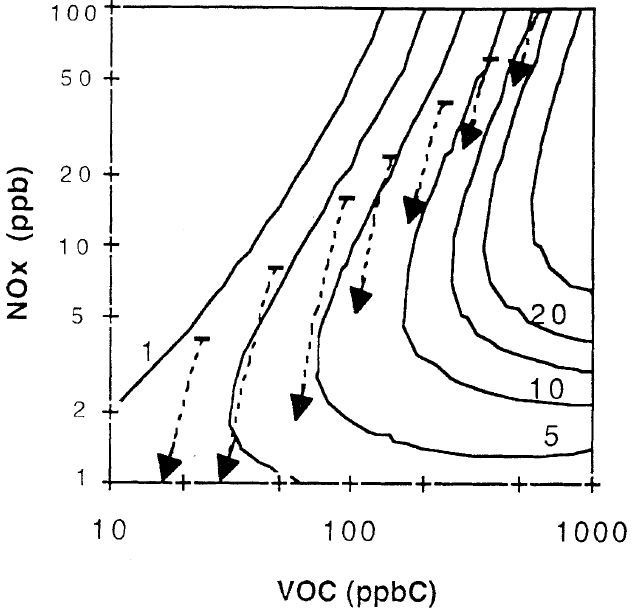
\includegraphics[height=80mm, width=75mm]{air_parcel.png}
		\caption{Air parcel evolution overlayed with ozone isopleth plots for various initial concentrations of \ce{NO_x} and VOCs. Taken from \citep{Sillman:1999}.}
		\label{f:air_parcel}
	\end{center}
\end{figure}
Once the air parcel has been emitted, it would typically fall into the VOC-sensitive regime but as the parcel ages it would 
move into the \ce{NO_x}-sensitive regime. Reducing VOC and \ce{NO_x} would reduce tropospheric \ce{O3}, whilst reducing VOC 
levels would only be effective during VOC-sensitive regimes and reducing \ce{NO_x} levels is only effective in 
\ce{NO_x}-sensitive regimes and can even increase \ce{O3} concentrations \citep{Sillman:1999}. This is due to the radical or 
\ce{NO_x} removal pathways that may or may not promote \ce{O3} production as discussed above.

Given the importance of determining the particular atmospheric regime at a specific time, a number of indicators that can be 
calculated from observational data have been determined. For example, in \citep{Kirchner:2001}, the parameter 
$\Theta = \tau^{\text{VOC}}_{\text{OH}} / \tau^{\ce{NO_x}}_{\text{OH}}$, where $\tau^{\text{VOC}}_{\text{OH}}$ is the lifetime 
of the OH radical against the loss by reaction with VOC and $\tau^{\ce{NO_x}}_{\text{OH}}$ is the lifetime of the OH radical 
against the loss by reaction with \ce{NO_x}. $\Theta$ can be used as such an indicator as it represents the relationship 
between the competing reactions of \ce{VOC + OH} and \ce{NO_x + OH}.

%ozone production rate P(O3)
Another measure of whether the atmosphere is in a VOC- or \ce{NO_x}-sensitive state is to calculate the chemical rate of 
\ce{O3} production, $P(\ce{O3})$. \citep{Kleinman:2005} derived an analytical formula for $P(\ce{O3})$ and showed that the rate 
of \ce{O3} production as a function of time is determined by $L_N/Q$, where $L_N$ is the rate of radical removal via reaction 
with \ce{NO_x} and $Q$ is the rate of radical production. $L_N/Q$ thus represents the fraction of free radicals that are 
removed with \ce{NO_x} and the remaining radicals being removed by addition reactions between free radicals.

\section{Ozone Production Potential}
%Ozone production potential of VOCs
The difficulty in applying uniform and successful emission control strategies due to the different regimes of the atmosphere 
has given rise to a more thorough investigation into the ozone production capabilities of different VOCs, also called the Ozone
Production Potential (OPP) of the VOC in question. This potential can be calculated via modelling studies and has given rise to
reactivity scales classifying the OPP of VOCs or classes of VOCs. The OPP of a VOC is dependent on the meteorological 
conditions, the reactivity of the VOC and the location of its emission. A wide range of such scales have been developed and are
discussed below.

\subsection{MIR and MOIR Incremental Reactivity Scales} \label{s:MIR&MOIR}
%Carter incremental reactivity scales
\citep{Carter:1994} outlines three incremental reactivity scales, the Maximum Incremental Reactivity (MIR), Maximum Ozone 
Incremental Reactivty (MOIR) and Equal Benefit Incremental Reactivity (EBIR) scales. The incremental reactivity of a VOC is 
defined as the change in \ce{O3} concentration caused when adding a small amount of the VOC in question to the emissions. 
Incremental reactivities are typically investigated through modelling studies although they can also be determined by means of 
airshed studies. 

The VOC reactivity, mechanism pathways and the atmospheric regime into which it is emitted all influence the incremental 
reactivity value of the VOC. Hence, the total \ce{NO_x} available is extremely important, as this determines the atmospheric 
regime present. For example, in VOC-sensitive regimes, the VOCs will have larger incremental reactivities than in a 
\ce{NO_x}-sensitive regime.

The MIR scale is calculated by adjusting the \ce{NO_x} levels so that the largest incremental reactivity was achieved for the 
individual VOC. The MOIR scale differs from the MIR as it is calculated using \ce{NO_x} levels that give the maximum ozone 
concentration for the whole VOC mix.  Whilst calculating the EBIR scale involves adjusting the \ce{NO_x} inputs so that the 
effect on \ce{O3} for a specific percentage change in VOC has the same effect of an equal percentange change in \ce{NO_x} 
\citep{Carter:1994}. The MOIR and EBIR scales are also shown in \citep{Carter:1994} to be practically equivalent when factoring 
in uncertainties during their calculation.

The MIR and MOIR scales are applicable to different regions due to their differences in \ce{NO_x} concentrations. The MIR scale
is applicable to places that have high transport emissions such as Los Angeles, as this implies an increased amount of 
\ce{NO_x} in the atmosphere when compared with the amount of VOCs. In contrast, the MOIR scale is more relevant to areas that 
have higher VOC (biogenic or anthropogenic) emissions. However, both scales do not include transport or multi-day scenarios 
during their calculation and this may effect their applicabilty \citep{Capps:2010}.

\subsection{Photochemical Ozone Creation Potential}
%POCP
The Photochemical Ozone Creation Potential (POCP) was introduced in \citep{Derwent:1996} and was used to calculate ozone 
production under the conditions applicable to northwestern Europe. This is in contrast to the MIR and MOIR which are both 
applicable to the US, due to the \ce{NO_x} levels used for their calculations and that in Europe the transport of reactive 
species and multi-day photochemistry are more important. Hence, the POCP values are calculated over a five day period.

The POCP is calculated by increasing the amount of a VOC in a photochemical trajectory model and calculating the increase in 
\ce{O3} concentration. This is then expressed as a percentage using the ozone increase due to the same amount in mass of ethene
as reference. The increased time period in the model runs  to calculate the POCP values showed that almost all VOC increase 
their ozone formation potential over time. The exceptions to this are the highly reactive VOC as they are completely oxidised 
during the initial emission phase \citep{Derwent:1996}. 

The calculation of the POCP was further refined in \citep{Derwent:1998} by using a more detailed chemical mechanism in the 
atmospheric model than that used in \citep{Derwent:1996} and by also studying the influence of different \ce{NO_x} 
concentrations. The Master Chemical Mechanism (MCM) is used as this provides a lot of chemical detail in the reaction 
mechanisms of the VOCs. 

The general trend of the POCP values did not change when using the MCM, however the individual values themselves were affected.
The \ce{NO_x} inputs were also adjusted in order to mirror planned changes in \ce{NO_x} emission standards and to investigate 
the robustness of these planned policies if based on POCPs. Once again, the same general trend of the POCP values was noted, 
although there are some VOCs (e.g. 1,3-butadiene) whose reactivity changed drastically depending on the \ce{NO_x} conditions 
\citep{Derwent:1998}. This again demonstrates the importance of taking into consideration the different possible regimes in the 
atmosphere as described in Section \ref{s:VOC&NOx}.

%use of IR scales
The use of incremental reactivity scales has been used in regulatory control in some US cities \citep{Luecken:2008}, where the 
MIR has mainly been used for such purposes. Due to the assumptions made during the generation of the scale itself, such as the 
\ce{NO_x} levels, it is not straightforward to extend the use of an incremental reactivity scale to a larger geographical area.
Moreover, the incremental reactivity scales are typically calculated using a box-model which does not include such factors as 
meteorology and may not include effects of transported air masses that, as previously discussed, can all influence the amount 
of \ce{O3} produced. 

%disadvantages of incremental reactivity scales 
A VOC's direct or indirect impact on ozone production cannot be distinguished when using incremental reactivity scales. The 
direct impact is the incremental effect of both the extra VOC and the resulting oxidation intermediates. Whilst the indirect 
impact is the effect that these VOC increments have on the availability of radical species which in turn influences the ozone 
production from other compounds in the base VOC mixture \citep{Butler:2011}, as discussed in Section \ref{s:VOC&NOx}. Another 
disadvantage is that the reactivity scales do not include detailed chemical information on the oxidation reactions of the VOC 
and how this is related to the OPP, moreover some scales do not account for the temporal effects of ozone production.

\subsection{Tagged Ozone Production Potential} \label{s:TOPP}
%TOPP
This led to a new approach outlined in \citep{Butler:2011} that links the degradation products of VOCs by using a tagging 
approach, called the Tagged Ozone Production Potential (TOPP). The calculation of the TOPP is taken over multiple days and 
calculates the direct impact of a particular VOC on its total impact on the \ce{O_x} family, defined previously in Section
\ref{s:reservoir}. The TOPP was calculated for NMVOCs listed in Table \ref{t:VOClist} and the atmospheric conditions related to
Los Angeles and Beijing and gave similar results despite these two cities having different NMVOC profiles. 

The TOPP values also indicate two groups of NMVOCs, those that reach a maximum in the first day of the simulation followed by a
decrease and those reaching a maximum TOPP after the first day. The first group includes many reactive NMVOCs such as alkenes 
and xylenes whilst the second group includes the slower reacting species such as alkanes and benzene. These groups can be 
determined as the time taken for a VOC to reach its maximum \ce{O3} production potential is dependent on the rate at which VOCs
yield smaller peroxy radical oxidation fragments. 

\citep{Butler:2011} also compares the TOPP to the MIR, MOIR and POCP showing that the TOPP compares well with all three, 
although to differing degrees for different classes of NMVOCs in the cases of the MIR and MOIR. An added advantage of the 
tagging approach used for the TOPP calculations is that the reaction pathways of the VOC in question that contribute to \ce{O3}
production can be determined. As in \citep{Butler:2011}, these reactions can be compared for different VOCs to determine the 
reactions that directly effect ozone production.

\section{Atmospheric Chemical Transport Models}
%Atmospheric models
Predictions of future \ce{O3} pollution levels are typically performed using mathematical atmospheric chemical transport 
models, these can be of different types depending on the study being performed. What is common between models is that they all 
must include an emission inventory, transport of the species, atmospheric physical and chemical transformation and numerical 
solutions to the applicable differential equations. 

Models are usually defined as either Eulerian or Lagrangian. The former describes the atmosphere in terms of fixed 
computational cells where species enter in and out of the cell walls and the concentrations of the species are then calculated 
as a function of time. Whilst the latter simulate changes of selected air parcels during advection through the atmosphere, 
hence there is no mass exchange between the surroundings and the air parcel (besides the emissions) and the model calculates 
concentrations at different locations at different times \citep{Seinfeld:2006}. Despite the differences that Eulerian and 
Langrangian models offer when undertaking a modelling study, Eulerian photochemical models constitute the majority of 
photochemical models (i.e. models dealing with atmospheric chemistry driven by photolysis as opposed to heterogeneous 
reactions) \citep{Russell:2000}.

Atmospheric models can also have different dimensions, ranging from zero-dimensional (also called a box model) to 
three-dimensional models. Box models have uniform atmospheric concentrations and are only a function of time, they are mainly 
used for focusing on the atmospheric chemistry or other detailed processes. Column models (or one-dimensional models) use 
concentrations that are a function of time and height, thus the grid is made up of many horizontally homogeneous layers. 
Two-dimensional models assume that concentration is constant in one direction and dependent on the other two directions and 
time. These models are used to describe global atmospheric chemistry with the assumption that concentration is a function of 
latitude and altitude but not longitude.  Three-dimensional models calculate concentration as a function of all three 
directions and time. Accuracy, simplicity and use of computing power all increase with the dimension of the model 
\citep{Seinfeld:2006}.

The model inputs may include meteorology, atmospheric concentrations (also used for initial and boundary conditions), 
emissions, topography and the grid structure \citep{Russell:2000}. Some models include online calculations of these inputs at 
each time step. Boundary conditions are typically the most difficult initial condition to set accurately as this requires 
knowledge of the investigated species concentrations at the boundary edges (if applicable) of the model grid. The model's 
dimension and type determine the set of differential equations that will be solved at each time step of the model run. 
Numerical methods are then used to solve the differential equations with the specified initial and boundary conditions. These 
methods vary between models and may be Runge-Kutta \citep{Sandu:1997b}, Finite Element \citep{Russell:2000} or Rosenbrock methods
\citep{Sandu:1997a}, to name three.

Setting the initial conditions involves fixing the starting concentrations of the species being studied, these conditions are 
dependent on the area being studied and whether it is an urban or rural area, amongst other considerations. The importance of 
setting the initial conditions depends on the model type, these conditions in Langrangian models are much more important than 
in Eulerian models, as this is the starting point at which the air parcel and its concentrations will be studied throughout the
model run. Boundary conditions are concentration flows of species and are important for both Eulerian and Lagrangian models. 
Emission inventories of the studied area are typically used, this is also believed to be one of the more uncertain inputs in a 
modelling study \citep{Russell:2000}.

\section{Chemical Mechanisms}
%Mechanisms in models
Models use chemical mechanisms to implement the atmospheric chemistry at each time step during a model run. The mechanism 
includes rate coefficients, reaction pathways with the corresponding branching ratios, photolysis rates and reaction products, 
amongst other parameters. This part of a model consumes a great deal of the computing resources, hence, when using a 
three-dimensional model the mechanism will include less chemical detail compared to a study incorporating a box-model. To 
achieve this, mechanisms used primarily in three-dimensional models will aggregate compounds, include more assumptions about 
how reactions proceed and how the degradation products are treated when compared to mechanisms used in box-modelling studies.

The Master Chemical Mechanism (MCM) in \citep{Saunders:2003, Jenkin:2003} is a near-explicit mechanism that is used for box 
modelling studies. Regional and global mechanisms include the Regional Atmospheric Chemistry Mechanism (RACM), the Carbon Bond 
Mechanism (CB-05 in \citep{Yarwood:2005}), the National Center for Atmospheric Research (NCAR) master mechanism 
(\citep{Madronich:1989}) and the Statewide Air Pollution Research Center (SAPRC), although many mechanisms include reduced 
mechanisms that are applicable to different model dimensions. A brief discussion of these mechanisms are included in 
\citep{Russell:2000} whilst the MCM, RACM and SAPRC mechanisms are discussed in more detail below.

\subsection{Self-Generating Mechanisms}
%self-generating mechanism
The self-generating mechanism is the type of chemical mechanism that reflects the details of the atmospheric chemistry 
summarised in Section \ref{s:atmo_chem} the most and is also called an explicit mechanism. This requires thousands of reactions
as the degradation of minor products is often more complex than that of the parent VOC. It also represents a compact method of 
obtaining a detailed mechanism that describes tropospheric chemistry.

\citep{Aumont:2005} outlines a way of including all reaction pathways that does not imply manually writing all the reactions 
with their respective parameters, as is the case for other mechanisms. This would also include the possibilty of heterogeneous 
chemistry and aerosol formation being accouted for in the mechanism, these are aspects of atmospheric chemistry that are not 
treated in great detail in chemical mechanisms used for gas-phase calculations.

The approach in \citep{Aumont:2005} is to write a so-called `generator' program that analyses the chemical structure of the VOC 
being studied to determine the reactive sites which then give the reaction pathways. The generator then accesses another file 
which includes the available reaction parameters and the reaction products. Structure activity relationships (SARs) are used 
when no reaction parameters are available. A file is then created that contains the final reaction, it includes the reactants, 
products and rate coefficients amongst other information. This process is then repeated for the products until all the 
oxidation reactions have been completed.

There are a number of advantages of this type of mechanism over mechanisms that are manually written up reaction by reaction. 
Firstly, a self-generating mechanism is faster to write since there are less reactions that need to be written due to the use 
of a generator program. This also implies increased accuracy (less manually written reactions means less typographical errors) 
and also maintenance is much easier as far less code needs to be updated. Currently, this type of mechanism has not been used 
in relation to ozone production potential calculations. 

\subsection{Master Chemical Mechanism}
%MCM v3.2
The Master Chemical Mechanism (MCM) v3.2 is a near-explicit mechanism describing the chemical degradation of 107 non-aromatic 
VOCs in \citep{Saunders:2003} and 18 aromatic VOCs in \citep{Jenkin:2003}. In total the MCM v3.2 has 12,691 reactions including 
4351 organic compounds and 46 associated inorganic compounds. The MCM includes alkanes, alkenes, dienes, monoterpenes, 
aromatics, aldehydes and ketones amongst others, the complete list is found online (\url{http://mcm.leeds.ac.uk/MCM/}). The VOCs
were chosen in accordance with the UK National Atmospheric Emissions Inventory and include those that make up about 70\% of the 
mass emissions of unique species achieved.

Each primary VOC and each degradation product, is individually degraded until it is broken down to \ce{CO2}, CO or an organic 
product (or radical) already found in the MCM \citep{Jenkin:1997}. The main assumptions made to reduce the number of reactions 
and compounds in the MCM are given below and are taken from \citep{Jenkin:1997}.
\begin{enumerate}
    \item The number of product channels resulting from reaction with the OH radical is limited by disregarding those pathways 
        of low probability.
    \item Many permutation (i.e. self and cross) reactions of organic peroxy radicals are represented by a single parameterised
        reaction. This is particularly required as inclusion of all peroxy radical reactions would involve about 400,000 
        reactions.
    \item The degradation chemistry is simplified, especially for those ``side" products deemed to be minor.
\end{enumerate}
Figure \ref{f:MCM_scheme} shows the reaction pathways represented in the MCM of a primary VOC, these shall be summarised below.
First the schemes used for the degradation reactions of non-aromatic VOCs in \citep{Saunders:2003} shall be discussed. As 
mentioned above, the main reaction pathway for VOC degradation is by OH radical reaction and hence this is included for the 
vast majority of VOCs considered. Reaction with \ce{O3} is deemed to only be important for alkenes, dienes, monoterpenes and 
some unsaturated oxygenated products. Reaction with the \ce{NO3} radical is mainly important during the night-time and for 
alkenes, dienes, aldehydes and ethers.  

For all reactions in the MCM, rate coefficients are taken from literature, where available, if not then they are estimated 
using methods also described in literature (for example, via SAR and group reactivity (GR) methods). The branching ratios of 
all reactions are also taken or estimated from literature. The reactions with \ce{O3} and the \ce{NO3} radical are also 
included if the parent VOC has a rate of removal that is more than 1\% of its removal rate with the OH radical and its lifetime
with respect to reaction with \ce{O3} (or \ce{NO3}, accordingly) is less than $10^7$ seconds.
\begin{figure}
    \begin{center}
        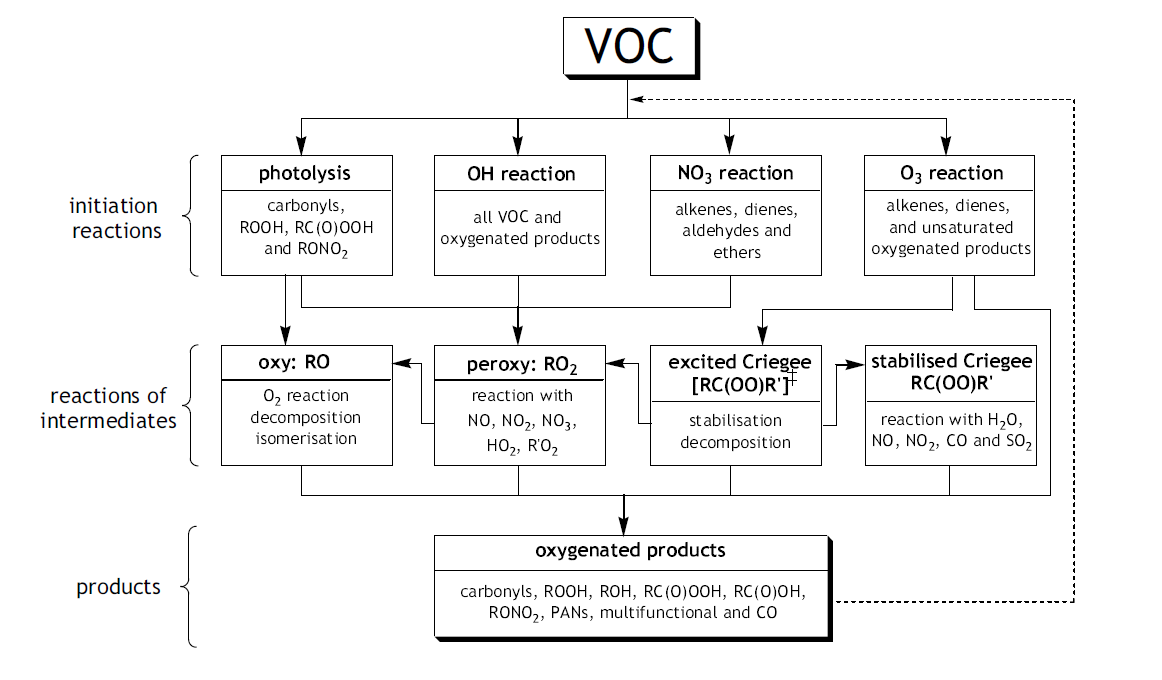
\includegraphics[width=13cm]{MCM_scheme.png}
        \caption{Flowchart of the major reactions, reactions of intermediates and products considered in the MCM. Taken from \citep{Saunders:2003}}
        \label{f:MCM_scheme}
    \end{center}
\end{figure}

Photolysis is included for those compounds that absorb at wavelengths less than 290 nm. The photolysis parameters are given for
those  compounds for which absorption cross-sections and quantum yield data is known and they are also determined as a function
of the solar zenith angle. 

The degradation products are also treated in detail, these first generation products are also degraded further as part of the 
MCM. Those products that have significant tropospheric concentrations are already treated in the MCM. To simplify this part of 
the mechanism, the products are limited to their reaction pathways with the OH radical. Those products which are deemed as 
minor are also greatly simplified whilst retaining product lifetimes and maintaining the carbon and nitrogen balance. However, 
many of these reactions are unbalanced in their \ce{O2} or \ce{H2O} output \citep{Jenkin:1997}. The kinetic data, where 
available, is taken from literature however mainly SAR estimations are used due to the lack of data.

In \citep{Jenkin:2003} the treatment of the aromatic VOCs included in the MCM v3.2 is described, this is summarised below. Where
possible the treatment follows that of non-aromatic VOCs as outlined above and in \citep{Saunders:2003}. However this is not 
possible for many reactions due to the intricacies of aromatic VOC chemistry and the fact that there is a lack of knowledge of 
the detailed degradation schemes. Also, similar simplifications are again present to reduce the complexity of the mechanism, 
this is particularly true for the \ce{C6 - C11} aromatic compounds.

Reaction with the OH radical is the main reaction pathway of aromatic compounds, the relevant rate coefficients are taken from 
literature, where available, or estimated depending on the functional group \citep{Jenkin:2003}. The reaction pathways are known
to proceed by H-atom abstraction or by addition to the aromatic ring. The branching ratios are taken from literature or applied
from the analogous molecule for which there is information. H-atom abstraction is typically deemed to be a minor pathway, at 
this point the simplification applied is that only one pathway during the initial OH radical attack is chosen. Literature 
provides the data at which point in the aromatic ring the addition reaction occurs and also the following reaction with 
\ce{O2}. Some specific cases are treated separately according to the relevant literature \citep{Jenkin:2003}.

The previous conditions outlined above for reaction with \ce{O3} and with the \ce{NO3} radical are also applied to aromatics 
VOCs. Again, all rate coefficients and branching ratios are either taken or estimated from the available data and the reaction 
pathways also proceed as described in literature. Photolysis is only considered for some aromatic VOCs based on the conditions 
described above. For those cases in which data are not available, the photolysis rates are taken by extension of the data 
available \citep{Jenkin:2003}. Hence, all reactions proceed as described in literature with estimations used for those cases 
lacking data.

The degradation products are also further degraded in the MCM, these are split into two general groups - those still containing
an aromatic ring and those formed after ring-opening. The latter are then treated as non-aromatic compounds as described above 
in \citep{Saunders:2003}. The former group is then further divided into four categories depending on the resulting product and 
these are then degraded according to \citep{Jenkin:2003}.

\subsection{Regional Atmospheric Chemistry Mechanism}
%RACM
Another chemical mechanism is the Regional Atmospheric Chemistry Mechanism (RACM), described in \citep{Stockwell:1997} and 
described below. This is a complete revision of the Regional Acid Deposition (RADM2) mechanism and is applicable to regional 
modelling and capable of simulating the gas phase tropospheric chemistry over remote and heavily polluted urban regions, 
including at the Earth's surface and in the upper troposphere. The RACM includes 17 inorganic, four inorganic intermediates and
32 organic species, four of which are of biogenic origin that altogether entail about 237 reactions. The inorganic reactions 
are practically fully described with the relevant rate coefficients, quantum yields and photolysis coefficients taken from 
literature.

In order to reduce computational resources for the mechanistic part of a regional model, the organic compounds are grouped into
16 anthropogenic and three biogenic model species. This grouping is based upon emission rates, functional group similarity and 
OH radical reactivity. Obtaining the final model species was done in two steps, first the hundreds of anthropogenic VOCs were 
grouped into 32 emission categories and then these were aggregated into the final 16 model species. Another aspect of reducing 
computational requirements was achieved by reducing the number of reaction pathways by only taking one reaction pathway from 
those available and also not treating all the organic intermediates explicitly.

The reaction rate coefficients of the model species are obtained by a weighted mean of all the rate coefficients of the organic
species aggregated into the model species, this is done to account for the difference in reactivities between the model and 
chemical species. The individual rate coefficients are taken from literature or estimated by means of a SAR. Some organic 
compounds (for example, methane and ethene) are explicitly treated, if not then the compounds are represented by a model 
species. For example, excluding ethene, anthropogenic alkenes with their double bond at the end of the molecule are included as
the model species as OLT whilst anthropogenic alkenes with their double bond not at the end of the molecule are represented by 
OLI \citep{Stockwell:1997}.

The different functional groups in a model species give rise to different reaction products, hence other model species are 
introduced with the relevant product yield fractions, as illustrated in the below reactions.
\begin{reactionlist}
    \reactionitem{OLT + OH}{OLTP}{new}{r:OLT+OH}
    \reactionitem{OLI + OH}{OLIP}{new}{r:OLI+OH}
\end{reactionlist}
These product species are calculated as a weighted mean of the product yields of all the chemical species represented by the 
model species, where the individual yields are taken from literature. 

The branching ratios of certain reactions are also parameterised, for example the slow-reacting aromatic species, represented by
the model species TOL, are assumed to react with the OH radical by addition to the aromatic ring with a 0.1 fraction of the 
reactions proceeding by H-atom abstraction.
\begin{reactionlist}
    \reactionitem{TOL + OH}{0.90 ADDT + 0.10 \ce{XO2} + 0.10 \ce{HO2}}{new}{r:TOL+OH}
\end{reactionlist}
Furthermore, the branching ratios of the reactions of the aromatic-OH adduct (ADDT) are determined by simulating the 
environmental chamber data and this calculation is dependent on the secondary products formed from the reactions of unsaturated 
dicarbonyls. This is a source of uncertainity in the mechanism and since these three pathways after the \ce{O3} production rate,
obtaining the correct branching ratio is of importance \citep{Stockwell:1997}.

The model species \ce{XO2} is used to represent peroxy radicals where the appropriate \ce{XO2} radical is dependent on the rate 
coefficient of the generating reaction. Also, the product yields are once again obtained via a weighted mean of the product 
yields of the individual species. To paramaterise the vast amount of reactions, very fast reactions are ignored and reactions 
with \ce{O3} are estimated due to the lack of experimental data. 

\citep{Kirchner:1996} details the treatment of organic peroxy radicals. The organic-peroxy radical-organic peroxy radical 
reactions are represented by reactions of the organic-peroxy radical with the two most important peroxy radicals (\ce{CH3O2} and
\ce{CH3C(O)O2}) and all other reactions with organic-peroxy radicals are ignored. The reaction rate coefficients of 
organic-peroxy radical self and cross reactions were estimated using the method described in \citep{Kirchner:1996}. Experimental 
data is used for the rate coefficients of alkyl peroxy radicals reaction with NO. 

\section{Comparison of Chemical Mechanisms}
%comparison of mechanisms
Given the different chemical mechanisms and their differing approaches towards simplifying the complexities of atmospheric 
chemistry, there have been many comparative studies to determine the differences between calculation results obtained when 
performing the same modelling study but altering the mechanism. In \citep{Dunker:1984} four mechanisms that were used in 
atmospheric modelling studies were compared by means of atmospheric simulations of box, trajectory and grid modelling studies 
and also against chamber study results. The comparison parameters were plotted \ce{O3}, \ce{NO2} and PAN isopleths as well as 
the time span required for the maximum one hour average \ce{O3}, \ce{NO2} and PAN concentrations to be reached. The largest 
differences between the mechanisms were found during the box model study whereas the other simulations correlated well. It is 
also highlighted that differences in chemistry can be masked by the effects of the meteorology and other parameters not included
in a box model.

A study of the chemical mechanisms used mainly for European regional studies are compared in \citep{Gross:2003}. Here, a box 
model study with the three different mechanisms is used to generate the concentrations of \ce{O3}, NO, \ce{NO2}, \ce{OH} 
radical, \ce{HO2} radical and organic peroxy radicals \ce{RO2}. \ce{O3} isopleth plots are also generated by performing the 
study over a range of \ce{NO_x} and VOC concentrations. A common set of photolysis coefficients were used so that the results 
would mirror only differences in the chemistry, the study also accounted for both urban and rural conditions in separate model 
runs.

The results show that the greatest differences between these mechanisms are in the \ce{O3}, \ce{NO2} and \ce{RO2} radical 
concentrations. The differences in the \ce{O3} concentrations are linked to the discrepancies between the \ce{NO2} and \ce{RO2} 
concentrations as these are reactions that lead to \ce{O3} production or loss. This emphasises the importance of the treatment
of organic peroxy radicals, which is typically one of the major areas of difference between chemical mechanisms. The rural study
showed little difference in the comparison parameters whilst the urban study showed larger differences. This can be attributed 
to the complexity of the organic chemistry prevalent in urban areas. \citep{Gross:2003} recommends that many different urban 
scenarios be considered and that \ce{O3} isopleth plots giving the \ce{O3} concentration over a range of \ce{NO_x} and VOC 
values should be used for such mechanism comparison studies. 

\citep{Emmerson:2009} compares the gas-phase chemical mechanisms used in global models. Since the MCM contains more chemical 
details than the reduced schemes used in global models it is used as a reference to which these are compared. The comparison is 
performed by box model runs simulating a large number of scenarios that are characteristic of global situations - industrial, 
clean, cold and dry, hot and wet, biogenic and non-biogenic conditions. Moreover, a particular recorded event (where the data 
are taken from the summer 2003 TORCH campaign) is also simulated with all the models to determine how close the simulation 
results are to the actual recorded concentrations. 

The simulations were ran without heterogenous chemistry and all set to begin at midnight in order to investigate the effect of 
night-time chemistry, which would be affected most by not including heterogenous chemistry. The length of each simulation is 
five days as a compromise between very long and very short run times which can affect the chemistry in different ways. Long 
model runs would imply significant aging of the air masses that would drive the chemistry and very short model runs would not 
test the chemistry pertaining to the degradation products at all, hence a compromise needs to be found. Separate model runs were
also performed to determine differences in the inorganic chemistry, full chemistry and night-time chemistry.

The resulting concentrations of specific compounds were plotted and compared to verify where mechanistic differences arise. The 
little difference between inorganic chemistry regimes can be attributed to the differences between kinetic data supplied by 
IUPAC and JPL, whilst there are more differences between the full chemistry and night-time chemistry. The greatest differences 
in the organic chemistry is when biogenic compounds, such as isoprene, are considered and are present in larger concentrations. 
For the specific pollution event that was modelled, the greatest differences arise for the night-time chemistry and \ce{O3} 
concentrations.

Reactivity scales have also been used as comparison tool for chemical mechanisms, this was proposed as in a single number, they 
provide a lot chemical kinetic data. In \citep{Derwent:2010}, the MCM and SAPRC are compared by calculation of the POCP of 116 
organic compounds from the major atmospheric classes within both mechanisms. A series of photochemical trajectory model runs 
simulating a single day were performed, many parameters other than the mechanisms were adjusted as incremental reactivities are 
not solely geophysical measures but rely on many other parameters.

The MCM and the SAPRC were chosen for this study as they are near-explicit mechanisms with the main difference being in how they
treat the first generation products - the MCM continues in an explicit manner while the SAPRC uses aggregation techniques. In 
general, the POCP values correlate very well between the two mechanisms, with a small number of exceptions. These can be 
attributed to the lack of detailed understanding of the degradation reactions of these compounds. The good correlation of 
reactivities of the aromatic compounds merely indicates that both mechanisms treat aromatic compounds similarly rather than 
having a detailed knowledge of these degradation schemes.

A detailed look at the chemistry affecting different mechanisms used in air quality modelling is described in 
\citep{Stockwell:2012}, where a box modelling study is undertaken with near-explicit and aggregated chemical mechanisms. The 
model system used is the same as that used in \citep{Seefeld:1999} with only gas-phase chemistry and constant meteorological 
conditions.  Different model runs were also undertaken with different temperatures in order to determine the temperature 
dependency of model results. 

The study highlights that the temperature dependence of gas phase reactions is uncertain for both organic and inorganic 
compounds. Also, night-time chemistry is a major source of uncertainty. Other knowledge gaps include the rate coefficients of 
the reactions of organic peroxy radicals as well as the products resulting from these reactions, the detailed degradation of 
both aromatic and biogenic compounds.

